\documentclass[UTF8]{ctexart}
% 基本设置和必要宏包
\usepackage{geometry}
\geometry{a4paper,scale=0.8}

% 数学相关宏包
\usepackage{amsmath}
\usepackage{amssymb}
\usepackage{amsfonts}

\usepackage{mathtools}
\usepackage{amsbsy}
\usepackage{amstext}
\usepackage{wasysym}
\usepackage{stmaryrd}
\usepackage{mathrsfs}

% 图形和颜色
%\usepackage{xcolor}
\usepackage{graphicx}
\usepackage{subcaption}
\usepackage{caption}
\usepackage{float}


% 其他功能性宏包
\usepackage{titlesec}
\usepackage{fancyhdr}
\usepackage{setspace}
\usepackage{cite}
\usepackage{appendix}
\usepackage{listings}
\usepackage{pdfpages}
\usepackage{enumitem}
\usepackage{tabu}
\usepackage{threeparttable}
\usepackage{booktabs}
\usepackage{abstract}
\usepackage{multirow}


\usepackage{diagbox} 
% 设置全局字体
%\setCJKmainfont{SimSun} % 设置正文为宋体
%\setCJKsansfont{SimHei} % 设置无衬线字体为黑体

% 允许公式跨页
\allowdisplaybreaks[4]



\newcommand{\sihaoheiti}{\fontsize{14pt}\selectfont\heiti}

% 论文题目设置为三号黑体字,并居中
\newcommand{\threelargebf}{\fontsize{16pt}{19.2pt}\selectfont\heiti\centering}

% 一级标题设置为四号黑体字,并居中
\titleformat{\section}{\centering\fontsize{14pt}{16pt}\bfseries\heiti}{\thesection}{1em}{}

% 二级标题设置为小四号黑体字,左对齐
\titleformat{\subsection}{\fontsize{12pt}{14.4pt}\bfseries\heiti}{\thesubsection}{1em}{\raggedright}

% 三级标题设置为小四号黑体字,左对齐
\titleformat{\subsubsection}{\fontsize{12pt}{14.4pt}\bfseries\heiti}{\thesubsubsection}{1em}{\raggedright}

% 正文字体设置为小四号宋体字,并使用单倍行距
\renewcommand{\normalsize}{\fontsize{12pt}{14.4pt}\selectfont}
%\renewcommand{\baselinestretch}{3}
%\selectfont



%\linespread{5.0}%修改行距
% 图片文件夹
\graphicspath{{img/}}
\let\itemize\compactitem
\let\enditemize\endcompactitem
% 设置页面布局
\geometry{a4paper, left=2.5cm, right=2.5cm, top=3cm, bottom=3cm}
\setstretch{1.2}

\renewcommand{\arraystretch}{1.5}
\newcommand{\thickhline}{\noalign{\hrule height 1.2pt}} % 设置粗线的宽度
\newcommand{\thinhline}{\noalign{\hrule height 0.8pt}} % 设置细线的宽度

%%%% ===== 定理环境
\usepackage[amsmath,thref,thmmarks,hyperref]{ntheorem} % 定理宏包
%\theorempreskipamount1em % spacing before the environment
%\theorempostskipamount0em  % spacing after the environment
%\theoremstyle{plain}
%\theoremheaderfont{\normalfont\heiti}
%\theorembodyfont{\normalfont\kaishu}
%\theoremindent0em
%\theoremseparator{\hspace{0.2em}}
%\theoremnumbering{arabic}

\newtheorem{property}{性质}[section]
\newtheorem{definition}{定义}[section]
\newtheorem{lemma}{引理}[section]
\newtheorem{remark}{注记}[section]
\newtheorem{corollary}{推论}[section]
\newtheorem{example}{例}[section] 
\newtheorem{problem}{{问题}}

 \renewcommand{\abstractnamefont}{\normalfont\bfseries}  % 摘要标题字体:正常字体,粗体
\renewcommand{\abstracttextfont}{\normalfont\normalsize}     % 摘要内容字体:正常字体,小四号

% 设置页眉页脚
\pagestyle{fancy}
\fancyhf{}
\fancyfoot[C]{\thepage}
\renewcommand{\headrulewidth}{0pt}

% 设置标题格式
\titleformat{\section}{\centering\heiti\large}{\thesection}{1em}{}
\titleformat{\subsection}{\raggedright\heiti\normalsize}{\thesubsection}{1em}{}
\titleformat{\subsubsection}{\raggedright\heiti\normalsize}{\thesubsubsection}{1em}{}

% 设置摘要环境
%\newenvironment{myabstract}{
%	\begin{center}
%	\bfseries\zihao{-3} 摘要
%	\end{center}
%	\vspace{-0.5em} % 调整摘要与论文题目的距离
%	\normalsize
%}{
%}
% 设置附录环境
\renewcommand{\appendixname}{附录}
\renewcommand{\appendixpagename}{附录}

% 设置代码环境
\lstset{
	basicstyle=\small\ttfamily,
	keywordstyle=\color{blue},
	commentstyle=\color{green!70!black},
	stringstyle=\color{red},
	breaklines=true,
	numbers=left,
	numberstyle=\tiny,
	frame=tb,
	language=Python
}
\newcommand{\bbA}{\mathbb{A}}
\newcommand{\bbB}{\mathbb{B}}
\newcommand{\bbC}{\mathbb{C}}
\newcommand{\bbD}{\mathbb{D}}
\newcommand{\bbE}{\mathbb{E}}
\newcommand{\bbF}{\mathbb{F}}
\newcommand{\bbG}{\mathbb{G}}
\newcommand{\bbH}{\mathbb{H}}
\newcommand{\bbI}{\mathbb{I}}
\newcommand{\bbJ}{\mathbb{J}}
\newcommand{\bbK}{\mathbb{K}}
\newcommand{\bbL}{\mathbb{L}}
\newcommand{\bbM}{\mathbb{M}}
\newcommand{\bbN}{\mathbb{N}}
\newcommand{\bbO}{\mathbb{O}}
\newcommand{\bbP}{\mathbb{P}}
\newcommand{\bbQ}{\mathbb{Q}}
\newcommand{\bbR}{\mathbb{R}}
\newcommand{\bbS}{\mathbb{S}}
\newcommand{\bbT}{\mathbb{T}}
\newcommand{\bbU}{\mathbb{U}}
\newcommand{\bbV}{\mathbb{V}}
\newcommand{\bbW}{\mathbb{W}}
\newcommand{\bbX}{\mathbb{X}}
\newcommand{\bbY}{\mathbb{Y}}
\newcommand{\bbZ}{\mathbb{Z}}

\title{}
\author{}
\date{}

\begin{document}


\begin{titlepage}		
		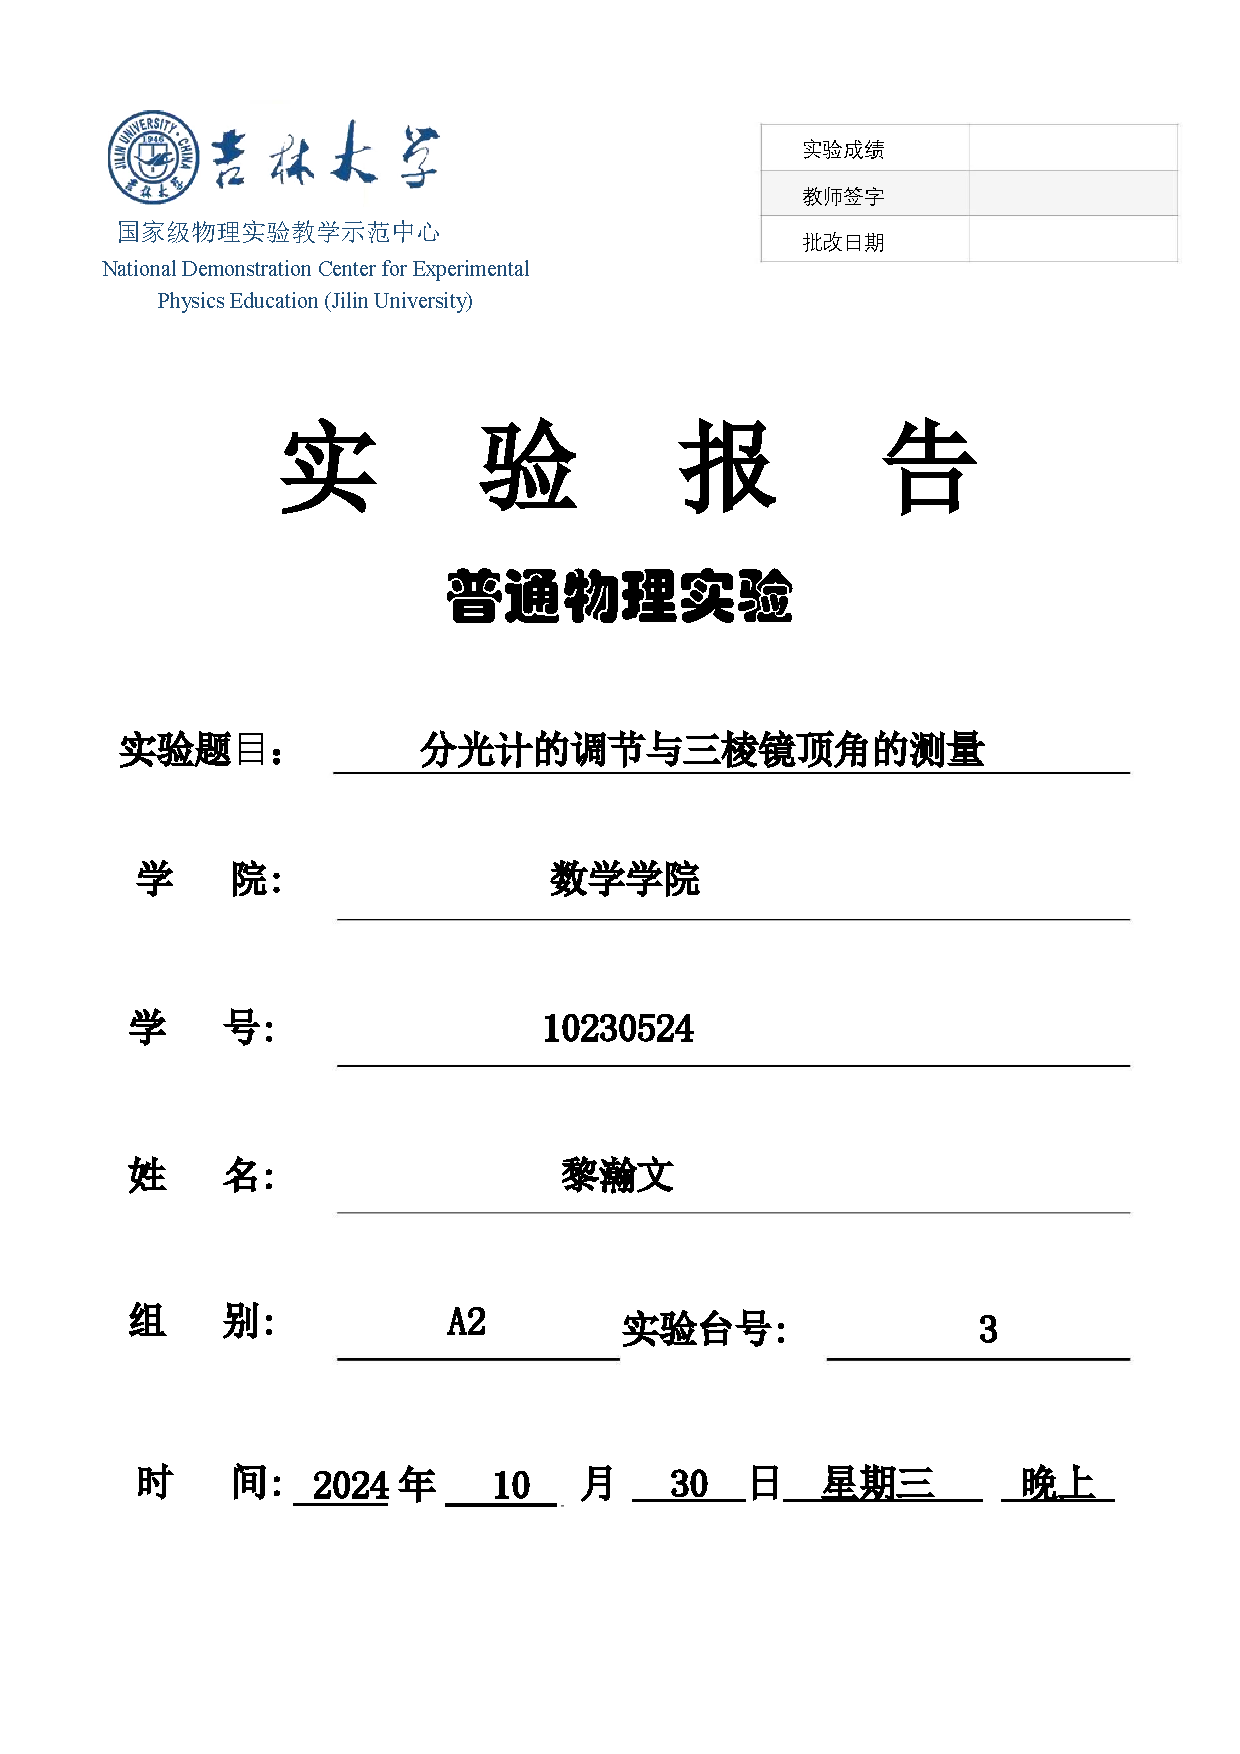
\includepdf[pages=-]{分光计封面.pdf}
\end{titlepage}

\section{实验过程}   % 这块实验内容占大头,都在上课讲,操作和细节上课认真听
\subsection{分光计的调节与三棱镜顶角的测量}
% 要求使用自己的语言描述实验过程,包括分光计的粗调、细调,三棱镜的调节的详细步骤和调节方法。每个步骤的操作方法要根据自己在实验过程中的体会进行详细描述。语言简捷,叙述清楚,内容全面。过于简略扣5-10分,照抄实验讲义或从网络上下载的扣10-15分

\textbf{粗调:}

首先固定望远镜下方的固定螺钉使望远镜在分光计调节过程中不发生移动,避免望远镜的移动造成偏差。

观察望远镜镜筒与平行光管是否平行,若出现明显不平行状态则调节望远镜下方的仰角螺钉和平行光管下方的仰角螺钉使其平行。关闭光源时,粗略调节望远镜使观察望远镜内最初出现浅绿色十字像

在调节望远镜时若非叉丝明显不清晰否则一般不移动接目镜

\textbf{细调:}

在粗调过程完成之后,首先调节载物台的两枚弹簧螺丝使其高度相等并首先确定两枚弹簧螺丝的高度,另一螺丝不做处理。

接着在载物台上放置一个两面小镜子模拟三棱镜旋转轴,以便调节望远镜光轴垂直于中心轴,调整使其位置大致与望远镜镜筒垂直,并且镜子其中一面与两枚固定弹簧螺丝连线平行,以便在望远镜视野里观察到反射像并能固定另一枚螺丝高度。

此时能在望远镜视野内观察到亮绿色十字像,更进一步若亮绿色十字像不在视野中心,则需旋转载物台调节使亮绿色十字像在视野中心。

再者需要调节望远镜下方的仰角螺丝与最初载物台上固定的两枚弹簧螺丝使得亮绿色十字像与最中心叉丝上方的叉丝重合。

使用“各调一半”的方法调节亮绿色十字像在镜子两面都与最中心叉丝上方的叉丝重合

在镜子一面内 在望远镜中估量亮绿色十字像与最上方叉丝的距离,并且调节望远镜下方的仰角螺钉使其移动到与亮绿色十字像距离的一半,再调节两枚载物台弹簧螺丝使亮绿色十字像与最中心叉丝上方叉丝重合;此时转动载物台使镜子另一面出现在视野内,观察是否出现亮绿色十字像。转动至亮绿色十字像出现在视野中心轴上时,估量其与最上方叉丝的距离并同样调节望远镜下方的仰角螺钉使其移动到与亮绿色十字像距离的一半,再调节两枚载物台弹簧螺丝使亮绿色十字像与最上方叉丝重合,此时再转动载物台到镜子第一面即视野中心轴内出现亮绿色十字像。重复上述操作直至镜子两面亮绿色十字像均与最上方叉丝重合。此时便调节望远镜光轴垂直于中心轴。


\textbf{三棱镜的调节}

平面镜调节完成后,将两面镜子换为三棱镜,并将三棱镜的三条边垂直螺钉连线放置如图,使磨砂面与细调时不调节的闲置螺钉在同一侧。转动载物台将三棱镜除磨砂面外的一面大致垂直于望远镜镜筒,并且使三棱镜中心与载物台中心大致重合。

此时转动载物台移动到三棱镜光滑面直至出现亮绿色十字像,同时只调节在该面的螺钉,使亮绿色十字像如细调一般与上方叉丝重合;转动载物台到另一光滑面,同样调节该面的螺钉使亮绿色十字像与上方叉丝重合,再转回原来一面。重复上述操作直至转动至两面光滑面时亮绿色十字像均与上方叉丝重合。


 \newpage
\textbf{三棱镜顶角的测量}

上述操作完成三棱镜调节后,转动三棱镜到其中一光滑面,亮绿色十字像与上方叉丝重合时,记录游标盘左右两个游标0刻度的读数 $\theta_1$ 和 $\theta_2$;转动至另一光滑面使亮绿色十字像与上方叉丝重合时,记录此时游标盘上述两个游标转动后0刻度的读数 $\theta'_1$ 和 $\theta'_2$。该过程中刻度盘与望远镜位置固定。

上述操作重复三次分别得到3组数据,使用公式  $\alpha = 180^{\circ} - \varphi $,其中$\varphi = \frac{1}{2}  \big[ (\theta'_1 - \theta_1 ) + (\theta'_2 - \theta_2 )\big]$,$\alpha$ 为三棱镜顶角,$\varphi$ 取其平均值。







\subsection{用最小偏向角测量介质的折射率}
%使用自己的语言描述实验过程,包括平行光管及狭缝的调节、最小偏向角及测量的详细步骤和调节方法。每个步骤的操作方法要根据自己在实验过程中的体会进行详细描述。语言简捷,叙述清楚,内容全面。过于简略扣2-4分,照抄实验讲义或从网络上下载的扣5分

将上述固定望远镜下方的固定螺钉拧松,使望远镜能够移动位置。

其次打开汞灯照亮平行光管的狭缝,并转动载物台以调节三棱镜使三棱镜与入射光线所成角度较小,此时转动望远镜找到经过三棱镜折射后的光线,找到使折射光线清晰的位置并使望远镜中心亮绿色叉丝集中在绿光上。

完成上述操作后,转动载物台使入射角改变,并使望远镜跟随其移动保证叉丝保持在绿光上。当转动到某一位置时折射光线朝着与移动方向相反的位置移动时,固定望远镜下方固定螺钉并转动载物台观察折射光线的变化,若确为反转点位置则记录该点处游标盘左右游标0刻度的读数 $\theta_3$ 和 $\theta_4$;转动载物台至另一折射面,使用与上述操作与测量同样的方法测量得到上述游标盘游标转动后对应游标0刻度的读数为 $\theta'_3$ 和 $\theta'_4$。

上述操作重复两次次分别得到2组数据

此时测量得到的角度为两折射面之间的夹角 $4 \delta_{min} $
$$ \delta_{min} = \frac{1}{4}  \big[ (\theta'_3 - \theta_3 ) + (\theta'_4 - \theta_4 )\big]$$

并将上述分光计求得的 三棱镜顶角$\alpha$ 与 求得的最小偏向角带入 $n = \frac{\sin \frac{\alpha + \delta_{min}}{2}}{\sin \frac{\alpha}{2}} $。 计算得到三棱镜对汞蓝线的折射率 $n$


\section{原始数据}

\begin{table}[H]
    \centering
    \caption{测量三棱镜顶角大小$\alpha$}
    \begin{tabular}{|c|c|c|c|c|c|c|c|}
    \toprule[1pt]
       组别  &   $\theta_1$ & $\theta_2$ & $\theta'_1$ & $\theta'_2$ & $\theta'_1 - \theta_1$ & $\theta'_2 - \theta_2$ & $\alpha$ \\
    \midrule
       1  &  $257^{\circ}8'$ & $77^{\circ}11'$ & $17^{\circ}7'$  &  $197^{\circ}15'$ & $119^{\circ}59'$ & $120^{\circ}4'$  & $59^{\circ}58'30''$\\
    \midrule
       2  & $257^{\circ}10'$  & $ 77^{\circ}12'$ & $17^{\circ}7'$  & $197^{\circ}17'$ & $119^{\circ}57'$  & $120^{\circ}5'$ & $59^{\circ}59'$\\
    \midrule
       3  & $257^{\circ}10'$ & $77^{\circ}12'$ & $17^{\circ}5'$  & $197^{\circ}15'$  &
       $119^{\circ}55'$  & $120^{\circ}3'$ & $60^{\circ}1'$ \\
    \bottomrule[1pt]
    \end{tabular}
\end{table}

\begin{table}[H]
    \centering
    \caption{测量三棱镜最小偏向角$\delta_{min}$}
    \begin{tabular}{|c|c|c|c|c|c|c|c|}
    \toprule[1pt]
       组别  &   $\theta_3$ & $\theta_4$ & $\theta'_3$ & $\theta'_4$ & $\theta'_3 - \theta_3$ & $\theta'_4 - \theta_4$ & $\delta_{min}$ \\
    \midrule
       1  &  $356^{\circ}13'$ & $176^{\circ}24'$ & $218^{\circ}53'$  &  $38^{\circ}48'$ & $137^{\circ}20'$ & $137^{\circ}16'$  & $68^{\circ}44'$\\
    \midrule
       2  & $353^{\circ}41'$  & $ 173^{\circ}50'$ & $216^{\circ}25'$  & $34^{\circ}49'$ & $137^{\circ}36'$  & $137^{\circ}1'$ & $68^{\circ}34'15''$\\
    \bottomrule[1pt]
    \end{tabular}
\end{table}

,









\section{数据处理}   % 没有不确定度的计算  % 但是评分主要在细节上
%  本实验的数据处理过程简单,不需要计算不确定度等,只需计算算数平均值即可。
%1.学生能够根据测得的实验数据,通过计算平均值给出三棱镜的顶角数值。
%2.学生计算过程要求采用度、分、秒的单位制,不能用小数点表述。
% 计算中出现的错误每处扣1分 


\subsection{三棱镜顶角的计算}

首先由于游标逆时针转动并过0刻度线,故测得的 $\theta'_1$  均需要加上 $360^{\circ}$;而$\theta_2 $本身测得与$\theta'_2 $ 为同一圈故直接相减即可。

则计算 $\theta'_1 - \theta_1$ 如下:
\begin{align*}
    (\text{组别为1}) \ \theta'_1 - \theta_1 &= 360^{\circ} + 18^{\circ}7' - 257^{\circ}8' = (377 - 257)^{\circ} + (67 - 8)' = 119^{\circ}59' \\
    (\text{组别为2}) \ \theta'_1 - \theta_1 &= 360^{\circ} + 18^{\circ}7' - 257^{\circ}10' = (377 - 257)^{\circ} +(67 - 10)' = 119^{\circ}57'
    \\
    (\text{组别为3}) \ \theta'_1 - \theta_1 &= 360^{\circ} + 18^{\circ}5' - 257^{\circ}10' = (377 - 257)^{\circ} + (65 - 10)' = 119^{\circ}55'
\end{align*}
\begin{align*}
    (\text{组别为1}) \ \theta'_2 - \theta_2 &=   197^{\circ}15' - 77^{\circ}11' = (197 - 77)^{\circ} + (15 - 11)' = 120^{\circ}4' \\
    (\text{组别为2})\ \theta'_2 - \theta_2 &=   197^{\circ}15' - 77^{\circ}11' = (197 - 77)^{\circ} + (17 - 12)' = 120^{\circ}5' \\
    (\text{组别为3}) \ \theta'_2 - \theta_2 &=   197^{\circ}15' - 77^{\circ}11' = (197 - 77)^{\circ} + (15 - 12)' = 120^{\circ}3' 
\end{align*}
\begin{align*}
    (\text{组别为1}) \ \varphi_1 &= \frac{1}{2} \big[ (\theta'_1 - \theta_1) + (\theta'_2 - \theta_2) \big]   \\
     &= \frac{1}{2} \times ( 119^{\circ}59' + 120^{\circ}4') =  \frac{1}{2} \times \big( ( 119 + 120)^{\circ} + ( 59 + 4)'   \big)  = \frac{1}{2} \times 240^{\circ}3' = 120^{\circ}1'30''\\
     \alpha_1 &= 180^{\circ} - \varphi_1 = 59^{\circ}58'30'' \\
    (\text{组别为2})\ \varphi_2 &= \frac{1}{2} \big[ (\theta'_1 - \theta_1) + (\theta'_2 - \theta_2) \big]   \\
     &= \frac{1}{2} \times ( 119^{\circ}57' + 120^{\circ}5') =  \frac{1}{2} \times \big( ( 119 + 120)^{\circ} + ( 57 + 5)'   \big)  = \frac{1}{2} \times 240^{\circ}2' = 120^{\circ}1'\\
     \alpha_2 &= 180^{\circ} - \varphi_2 = 59^{\circ}59' \\
    (\text{组别为3})\ \varphi_3 &= \frac{1}{2} \big[ (\theta'_1 - \theta_1) + (\theta'_2 - \theta_2) \big]   \\
     &= \frac{1}{2} \times ( 119^{\circ}55' + 120^{\circ}3') =  \frac{1}{2} \times \big( ( 119 + 120)^{\circ} + ( 55 + 3)'   \big)  = \frac{1}{2} \times 239^{\circ}58' = 119^{\circ}59' \\
      \alpha_3 &= 180^{\circ} - \varphi_3 = 60^{\circ}1' 
\end{align*}
\begin{align*}
    \overline{\alpha} &= \frac{\alpha_1 + \alpha_2 + \alpha_3}{3}  \\
    &= \frac{59^{\circ}58'30'' +  59^{\circ}59' + 60^{\circ}1'}{3} = \frac{1}{3} \big( (59 + 59 + 60)^{\circ} + (58 + 59 + 1)'+ (30)''  \big)  \\
    &= \frac{1}{3} \times 179^{\circ}58'30'' = 59^{\circ}59'30''
\end{align*}


\subsection{三棱镜折射率的计算}
由于转动望远镜时为顺时针转动,故$\theta'_3$ 和 $\theta'_4$ 测得读数均比$\theta_3$ 和 $\theta_4$ 更小且在同一圈内。故相减时取其绝对值。
\begin{align*}
    (\text{组别为1}) \ \theta'_3 - \theta_3 &= | 218^{\circ}53' - 356^{\circ}13'| = (355 - 218)^{\circ} + (73 - 53)' = 137^{\circ}20' \\
    (\text{组别为2}) \ \theta'_3 - \theta_3 &= | 216^{\circ}25' - 353^{\circ}41'| = (353 - 216)^{\circ} + (41 - 25)' = 137^{\circ}16' 
\end{align*}
\begin{align*}
    (\text{组别为1}) \ \theta'_4 - \theta_4 &= | 38^{\circ}48' - 176^{\circ}24'| = (175 - 38)^{\circ} + (84 - 48)' = 137^{\circ}36' \\
    (\text{组别为2}) \ \theta'_4 - \theta_4 &= | 34^{\circ}49' - 173^{\circ}50'| = (173 - 34)^{\circ} + (50 - 49)' = 137^{\circ}1' 
\end{align*}
\begin{align*}
    (\text{组别为1}) \ \delta_{min}^{(1)} &=  \frac{1}{4} \big( (\theta'_3 - \theta_3 ) + (\theta'_4 - \theta_4) \big)\\
    &= \frac{1}{4} \times (137^{\circ}20' + 137^{\circ}36') = \frac{1}{4} \times 274^{\circ}56' = 68^{\circ}44' \\
    (\text{组别为2}) \ \delta_{min}^{(2)} &=  \frac{1}{4} \big( (\theta'_3 - \theta_3 ) + (\theta'_4 - \theta_4) \big)\\
    &= \frac{1}{4} \times (137^{\circ}16' + 137^{\circ}1') = \frac{1}{4} \times 274^{\circ}17' = 68^{\circ}34'15'' 
\end{align*}
\begin{align*}
    (\text{组别为1}) \ n_1  = \frac{\sin \frac{  \overline{\alpha} + \delta_{min}^{(1)}}{2}}{\sin \frac{\overline{\alpha}}{2}}  = 
    \frac{\sin \frac{  59^{\circ}59'30'' +  68^{\circ}44'}{2}}{\sin \frac{59^{\circ}59'30''}{2}} =  1.8089 \\
    (\text{组别为2}) \ \ n_2  = \frac{\sin \frac{\overline{\alpha} + \delta_{min}^{(2)}}{2}}{\sin \frac{\overline{\alpha}}{2}} = \frac{\sin \frac{  59^{\circ}59.5' +  68^{\circ}34'15''}{2}}{\sin \frac{59^{\circ}59'30''}{2}} = 1.8082 
\end{align*}
\begin{align*}
 \overline{\delta_{min}} &= \frac{\delta_{min}^{(1)} + \delta_{min}^{(2)}}{2} = \frac{68^{\circ}44' + 68^{\circ}34'15'' }{2} = 68^{\circ}39'8'' \\
    \overline{n} &= \frac{n_1 + n_2}{2} =   \frac{1.8089 + 1.8082}{2} = 1.80855
\end{align*}





\newpage
\section{结果分析}
%实验结果比较分析或实验心得 
分光计调节与三棱镜顶角测量实验中测量得到的三棱镜顶角为 $59^{\circ}59'30''$,与三棱镜纵切面为等边三角形的顶角 $60^{\circ}$ 误差为 $30''$,测量得到数据较为精确。

测量三棱镜折射率实验中测得的最小偏向角为 $\delta_{min} = 68^{\circ}39'8''$,与实验室实际三棱镜最小偏向角 $70^{\circ}$,差距 为 $1^{\circ}20'52''$,差距较小在合理范围内。数据测量不够准确的原因可能为:实验中调节的光缝大小与理想状态有偏差导致折射光线的宽度有误差;或者为转动载物台时未能更加精确地确认最小偏向角的位置,导致测得恰好反向的位置偏小。

\section{实验心得}

实验过程中老师对于分光计的调节和测量三棱镜折射率实验中步骤的讲解对于完成实验有较大帮助,具体听讲与分析比课本上的内容更加具体,实验后明显提高了对实验的了解程度和器材的熟练程度。

\section{思考题}
\subsection{分光计的调节与三棱镜顶角的测量}
\subsubsection{实验数据产生误差的因素}
\begin{enumerate}
    \item 仪器误差:分光计的分度盘分辨率有限,刻度的最小读数决定了角度测量的精度;三棱镜的顶角可能并非完全理想值而存在微小的加工误差,这样的误差在角度测量中可能会累积
    \item 对准误差:亮绿色十字像与上方叉丝重合时存在模糊位置区间,可能导致读数产生偏差;以及读数时肉眼产生的游标上的微小偏差。
\end{enumerate}
\subsubsection{调节望远镜光轴与分光计中心轴垂直时使用各调一半法的原因以及使用各调一半法的方法}
原因有:
\begin{enumerate}
    \item 通过“各调一半”的方法,可以均匀分配调整误差,避免单次大幅度调整带来的偏差。各调一半法将误差平均分摊到望远镜和分光计的两部分,有助于更精准地对准分光计的中心位置,使得光路和中心轴重合。
    \item 如果单独调节一端,可能会因单边调节过多使调节时无论如何也调节不到二者亮绿色十字像与上方叉丝重合的位置。
\end{enumerate}

方法:将望远镜和分光计都调整到一个初始位置,观察光轴的偏离程度,先对望远镜和分光计进行粗略调节,使其大致处于垂直状态;然后调节三棱镜该面载物台螺钉与望远镜螺钉各自调节亮绿色十字像与上方叉丝距离的一半,其次转动载物台到另一面重复上述操作。重复上方操作直到转到载物台在三棱镜两面都能看到亮绿色十字像与上方叉丝重合。

\subsubsection{三棱镜放置在载物台上时为什么载物台上有一个螺丝不需要调节的原因}
为了使三棱镜稳固放置,载物台的三个支点决定了它的平面位置。根据几何原理,三个支点可以唯一确定一个平面,因此只需要调节其中的两个螺丝就可以达到调整平面的目的,第三个螺丝起到稳定支撑的作用而不需要调节。同时可以减少调节的复杂性,避免多次反复调整,提高实验效率
\subsubsection{分光计的主要部件组成与各自作用}
分光计的主要部件有:三角底座、望远镜、平行光管、载物台和读数圆盘。

作用:

\begin{enumerate}
    \item 三角底座:底座用于支撑整个分光计装置,确保仪器的稳定性和水平状态
    \item 望远镜:用于观察进入分光计的光线。通过望远镜可以看到光的折射、反射或色散后的像,并测量光线经过棱镜或其他光学器件时发生的偏转角
    \item 平行光管:产生平行光
    \item 载物台:用于放置光学元件,如三棱镜。可旋转并具有刻度标记,以便精确调整和记录光学元件的位置
    \item 读数圆盘:记录光线的入射角和折射角,帮助计算光的折射率或色散情况
\end{enumerate}
   


\subsection{用最小偏向角测量介质的折射率}

\subsubsection{确定最小偏向角的方法}
将光源的光线通过准直管准直后,入射到三棱镜的一侧表面,使光线经过折射和出射后进入望远镜。调整分光计,使光线偏向角约为较小值。缓慢转动三棱镜,同时观察望远镜中折射光线的位置。当偏向角逐渐减小时,继续缓慢转动三棱镜,直到观察到光线偏向角不再减小,并开始增大,此时光线达到了最小偏向角。

\subsubsection{调节狭缝和平行光管的方法}
调节狭缝:通过旋转狭缝调节旋钮,可以改变狭缝的宽度。通常应将狭缝宽度调到适中状态——足够窄以得到清晰的光谱线,但不至于太窄而导致光线过暗

调节平行光管:若已经使平行光管平行于望远镜,则必然垂直于中心轴,只需将缝像的中心点调到叉丝交点

\end{document}